% Co-Wingman research poster. Main file; compile with pdfLaTeX.
% All text and diagrams are editable. Images live in images/.
\documentclass{article}
\usepackage[paperwidth=48in,paperheight=36in,margin=0in]{geometry}
\usepackage[T1]{fontenc}
\usepackage[utf8]{inputenc}
\usepackage{helvet}
\renewcommand{\familydefault}{\sfdefault}
\usepackage{graphicx}
\usepackage{tikz}
\usetikzlibrary{arrows.meta,calc}
\usepackage{array}
\usepackage{hyperref}
\hypersetup{colorlinks=true,urlcolor=white,pdftitle={Co-Wingman Research Poster}}
\pagestyle{empty}
\setlength{\parindent}{0pt}

% ---------- DESIGN SETTINGS ----------
% Coordinates below use a 1448 x 1086 design grid (top-left origin).
% The entire design is scaled to the paper size declared above.
\definecolor{navy}{HTML}{07346A}
\definecolor{blue}{HTML}{0875B9}
\definecolor{orange}{HTML}{F36C21}
\definecolor{ink}{HTML}{172E42}
\definecolor{muted}{HTML}{4B6174}
\definecolor{panelbg}{HTML}{F5F9FD}
\definecolor{lineblue}{HTML}{BFD8EA}
\definecolor{localbg}{HTML}{EAF5FD}
\definecolor{cloudbg}{HTML}{EDF8EE}
\definecolor{green}{HTML}{18834B}
\definecolor{awsbg}{HTML}{FFF0E2}
\definecolor{awstext}{HTML}{9F430C}
\tikzset{
  flow/.style={-{Stealth[length=6pt,width=5pt]},line width=1.8pt,draw=blue},
  cloudflow/.style={flow,draw=green},
  awsflow/.style={flow,draw=orange},
  block/.style={anchor=center,rounded corners=5pt,draw=blue,fill=white,line width=.8pt,
    align=center,inner sep=5pt,font=\sffamily\fontsize{15}{17}\selectfont,text=ink}
}
\newcommand{\Text}[6]{% x,y,width,font-size,color,content
  \pgfmathsetmacro{\textleading}{1.18*(#4)}
  \pgfmathsetlengthmacro{\textwidthvalue}{(#3)*1pt}
  \node[anchor=north west,inner sep=0pt,text width=\textwidthvalue,text=#5,
    font=\sffamily\fontsize{#4}{\textleading}\selectfont] at (#1,#2)
    {\raggedright\hyphenpenalty=10000 #6\par};
}
\newcommand{\Panel}[5]{% x,y,width,height,title
  \filldraw[rounded corners=7pt,fill=panelbg,draw=lineblue,line width=.8pt]
    (#1,#2) rectangle ({#1+#3},{#2+#4});
  \begin{scope}
    \clip[rounded corners=7pt] (#1,#2) rectangle ({#1+#3},{#2+#4});
    \fill[navy] (#1,#2) rectangle ({#1+#3},{#2+42});
  \end{scope}
  \Text{#1+14}{#2+9}{#3-28}{22}{white}{\bfseries #5}
}
\newcommand{\Badge}[4]{% x,y,number,text
  \fill[blue] (#1,#2) circle[radius=13pt];
  \node[anchor=center,inner sep=0pt,text=white,font=\bfseries\fontsize{14}{16}\selectfont] at (#1,#2) {#3};
  \Text{#1+26}{#2-12}{205}{17}{ink}{#4}
}
% EDIT POSTER WORDING AND MEASUREMENTS HERE.
% Escape LaTeX special characters: \&, \%, \_, \#.
\newcommand{\PosterTitle}{Co-Wingman: A Hybrid Edge--Cloud AI Assistant\\
for Real-Time Conversational Recovery Cues}
\newcommand{\Authors}{Mrunal Vibhute, Shrimayee Deshpande, Honey Reddy Daram, Dr. Andrea Ramirez-Salgado}
\newcommand{\Affiliation}{University of Florida | Master's in AI Systems | AI Days 2026}
\newcommand{\Motivation}{Help speakers recover a thought with a short, context-aware cue during a conversational pause.}
\newcommand{\PrivacyText}{%
  Raw audio stays on the Jetson.\par\vspace{13pt}
  Only bounded text reaches UF NaviGator.\par\vspace{13pt}
  AWS storage is opt-in.\par\vspace{13pt}
  Pause assistance detects silence, not anxiety or speaker identity.}
\newcommand{\ResultsRows}{%
  ASR inference & 110 ms & 127 ms\\
  Cue handling & 1.04 s & 2.54 s\\
  Summary update & 1.42 s & 1.99 s\\}
\newcommand{\ResultsNote}{%
  Timing sample: pause-assist-05; photo from a separate demo.
  69 voiced windows, 7 summaries, zero recorded stage failures.
  Cue timing excludes capture wait; a completed request may offer no cue.}
\newcommand{\AWSStatus}{AWS integration implemented; live upload/reload validation pending.
  AWS was not included in this timing test.}
\newcommand{\NextSteps}{%
  \textcolor{orange}{\bfseries 1.}\ Reduce four-second buffering delay\\[5pt]
  \textcolor{orange}{\bfseries 2.}\ Evaluate cue usefulness with users\\[5pt]
  \textcolor{orange}{\bfseries 3.}\ Validate AWS upload and recovery\\[5pt]
  \textcolor{orange}{\bfseries 4.}\ Evaluate experimental disfluency scoring}


\begin{document}
\null
\begin{tikzpicture}[remember picture,overlay]
\node[anchor=north west,inner sep=0pt] at (current page.north west) {%
\resizebox{\paperwidth}{\paperheight}{%
\begin{tikzpicture}[x=1pt,y=-1pt]
\path[use as bounding box] (0,0) rectangle (1448,1086);
\clip (0,0) rectangle (1448,1086);
\fill[white] (0,0) rectangle (1448,1086);

% ---------- HEADER ----------
\Text{44}{10}{1113}{37}{navy}{\bfseries \PosterTitle}
\Text{48}{121}{1090}{22}{ink}{\Authors}
\Text{48}{153}{1085}{20}{ink}{\Affiliation}
\node[anchor=north west,inner sep=0pt] at (1172,14)
  {
\includegraphics[width=250pt,height=162pt,keepaspectratio]{images/hwcoe-logo.png}};
\fill[orange] (12,189) rectangle (1436,193);

% ---------- LEFT COLUMN ----------
\Panel{14}{205}{280}{232}{Motivation}
% Simple speech icon, editable TikZ.
\fill[blue] (65,313) circle[radius=25pt];
\fill[blue] (42,326) -- (38,358) -- (80,358) -- (75,330) -- cycle;
\draw[orange,line width=3pt] (95,313) to[bend left=35] (95,347);
\draw[orange,line width=2pt] (103,306) to[bend left=35] (103,354);
\Text{124}{275}{150}{18}{ink}{\Motivation}

\Panel{14}{447}{280}{333}{Prototype capabilities}
\Badge{43}{517}{1}{Local speech recognition}
\Badge{43}{565}{2}{Rolling 60-second context}
\Badge{43}{613}{3}{Manual or pause-triggered cues}
\Badge{43}{671}{4}{Optional portfolio grounding}
\Badge{43}{730}{5}{Minute summaries and S3 continuity}

\Panel{14}{790}{280}{241}{Privacy \& control}
\Text{30}{851}{248}{17}{ink}{\PrivacyText}

% ---------- CENTER: CONVERSATION ----------
\Panel{304}{205}{706}{332}{Speak \textrightarrow\ Pause \textrightarrow\ Recover}
% Keep the supplied generated conversation illustration as an image asset.
% It is clipped from its source in LaTeX; replace with your own illustration
% by changing this node. Text inside this illustration is part of the bitmap.
\begin{scope}
  \clip (311,253) rectangle (1004,530);
  \node[anchor=north west,inner sep=0pt] at (5,-1)
    {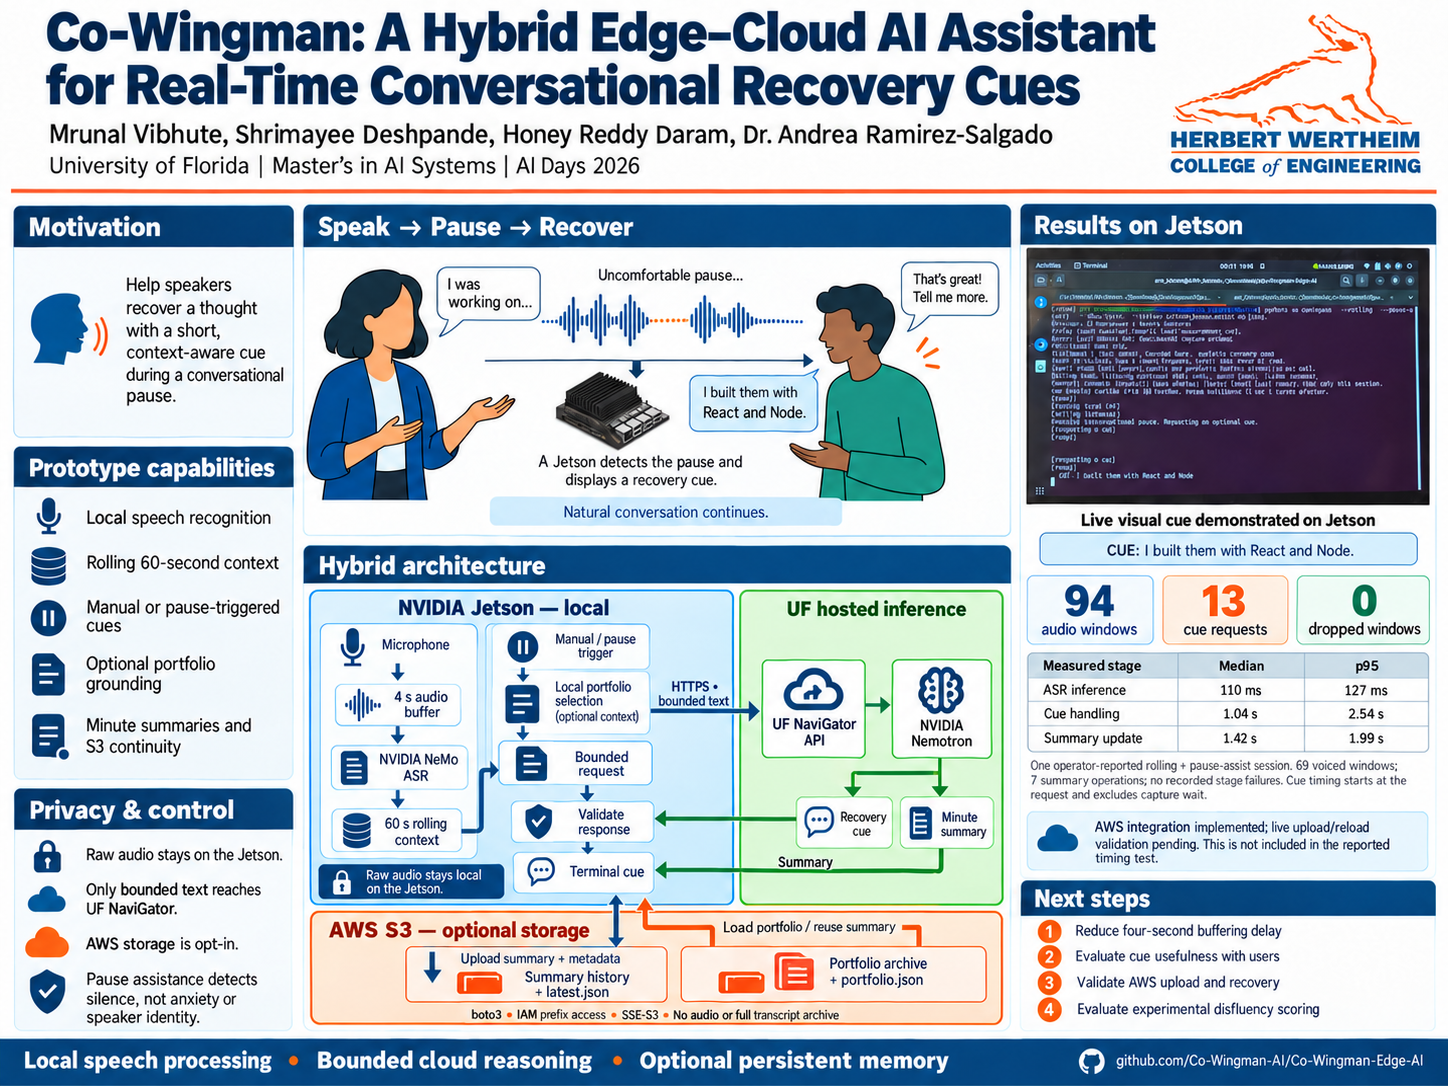
\includegraphics[width=1433pt]{images/conversation-reference.png}};
\end{scope}

% ---------- CENTER: EDITABLE TIKZ ARCHITECTURE ----------
\Panel{304}{547}{706}{484}{Hybrid architecture}
% EDITABLE ARCHITECTURE. Included inside the main TikZ picture.
% Blue = local Jetson; green = UF inference; orange = optional AWS storage.
\filldraw[rounded corners=7pt,fill=localbg,draw=blue,line width=1pt]
  (310,592) rectangle (733,903);
\filldraw[rounded corners=7pt,fill=cloudbg,draw=green,line width=1pt]
  (741,592) rectangle (1003,903);
\Text{321}{604}{400}{21}{navy}{\centering\bfseries NVIDIA Jetson -- local}
\Text{751}{604}{242}{21}{green}{\centering\bfseries UF hosted inference}

\node[block,minimum width=120pt,minimum height=58pt] (mic) at (389,681)
  {Microphone\\4 s audio buffer};
\node[block,minimum width=120pt,minimum height=58pt] (asr) at (522,681)
  {NVIDIA\\NeMo ASR};
\node[block,minimum width=120pt,minimum height=58pt] (context) at (655,681)
  {60 s rolling\\text context};
\draw[flow] (mic.east) -- (asr.west);
\draw[flow] (asr.east) -- (context.west);

\node[block,minimum width=120pt,minimum height=58pt] (trigger) at (389,770)
  {Manual / pause\\trigger};
\node[block,minimum width=120pt,minimum height=58pt] (portfolio) at (522,770)
  {Local portfolio\\selection};
\node[block,minimum width=120pt,minimum height=58pt] (request) at (655,770)
  {Bounded\\request};
\draw[flow] (context.south) -- (request.north);
\draw[flow] (portfolio.east) -- (request.west);
\draw[flow] (trigger.north) -- (389,726) -- (630,726) -- (630,741);

\node[block,draw=green,minimum width=214pt,minimum height=56pt] (api) at (872,751)
  {\bfseries UF NaviGator API};
\node[block,draw=green,minimum width=214pt,minimum height=56pt] (model) at (872,835)
  {\bfseries NVIDIA Nemotron\\\normalfont\fontsize{13}{15}\selectfont Cue / minute summary};
\draw[cloudflow] (request.east) -- (730,770) -- (730,751) -- (api.west);
\Text{715}{728}{48}{10}{green}{\centering HTTPS}
\draw[cloudflow] (api.south) -- (model.north);

\node[block,minimum width=188pt,minimum height=47pt] (validate) at (621,849)
  {Validate response};
\node[block,minimum width=169pt,minimum height=47pt] (terminal) at (413,849)
  {Terminal cue};
\draw[cloudflow] (model.west) -- (validate.east);
\draw[flow] (validate.west) -- (terminal.east);
\Text{321}{884}{400}{11}{navy}{\centering\bfseries Raw audio stays local. Rolling listening continues during cue calls.}

% S3 connects through the Jetson app, never directly to the hosted model.
\filldraw[rounded corners=7pt,fill=awsbg,draw=orange,line width=1pt]
  (310,927) rectangle (1003,1021);
\Text{324}{936}{660}{20}{awstext}{\bfseries AWS S3 -- optional storage}
\Text{341}{964}{295}{15}{ink}{\bfseries Summary history\quad\normalfont windows/ + latest.json}
\Text{656}{964}{330}{15}{ink}{\bfseries Portfolio archive\quad\normalfont portfolio.json}
\Text{324}{1001}{662}{11}{awstext}{\centering boto3\quad\textbullet\quad IAM prefix access\quad\textbullet\quad SSE-S3\quad\textbullet\quad No audio or full transcript archive}
\draw[awsflow] (485,903) -- (485,927);
\draw[awsflow] (704,927) -- (704,903);
\Text{314}{909}{165}{10}{awstext}{Upload summary + metadata}
\Text{514}{909}{186}{10}{awstext}{Load portfolio / reuse summary}


% ---------- RIGHT: RESULTS ----------
\Panel{1020}{205}{416}{666}{Results on Jetson}
% Original photograph, never re-created by image generation.
% Clipping removes desk/bezel; edit these coordinates to change the crop.
\begin{scope}
  \clip (1028,253) rectangle (1428,475);
  \node[anchor=north west,inner sep=0pt] at (1000,149)
    {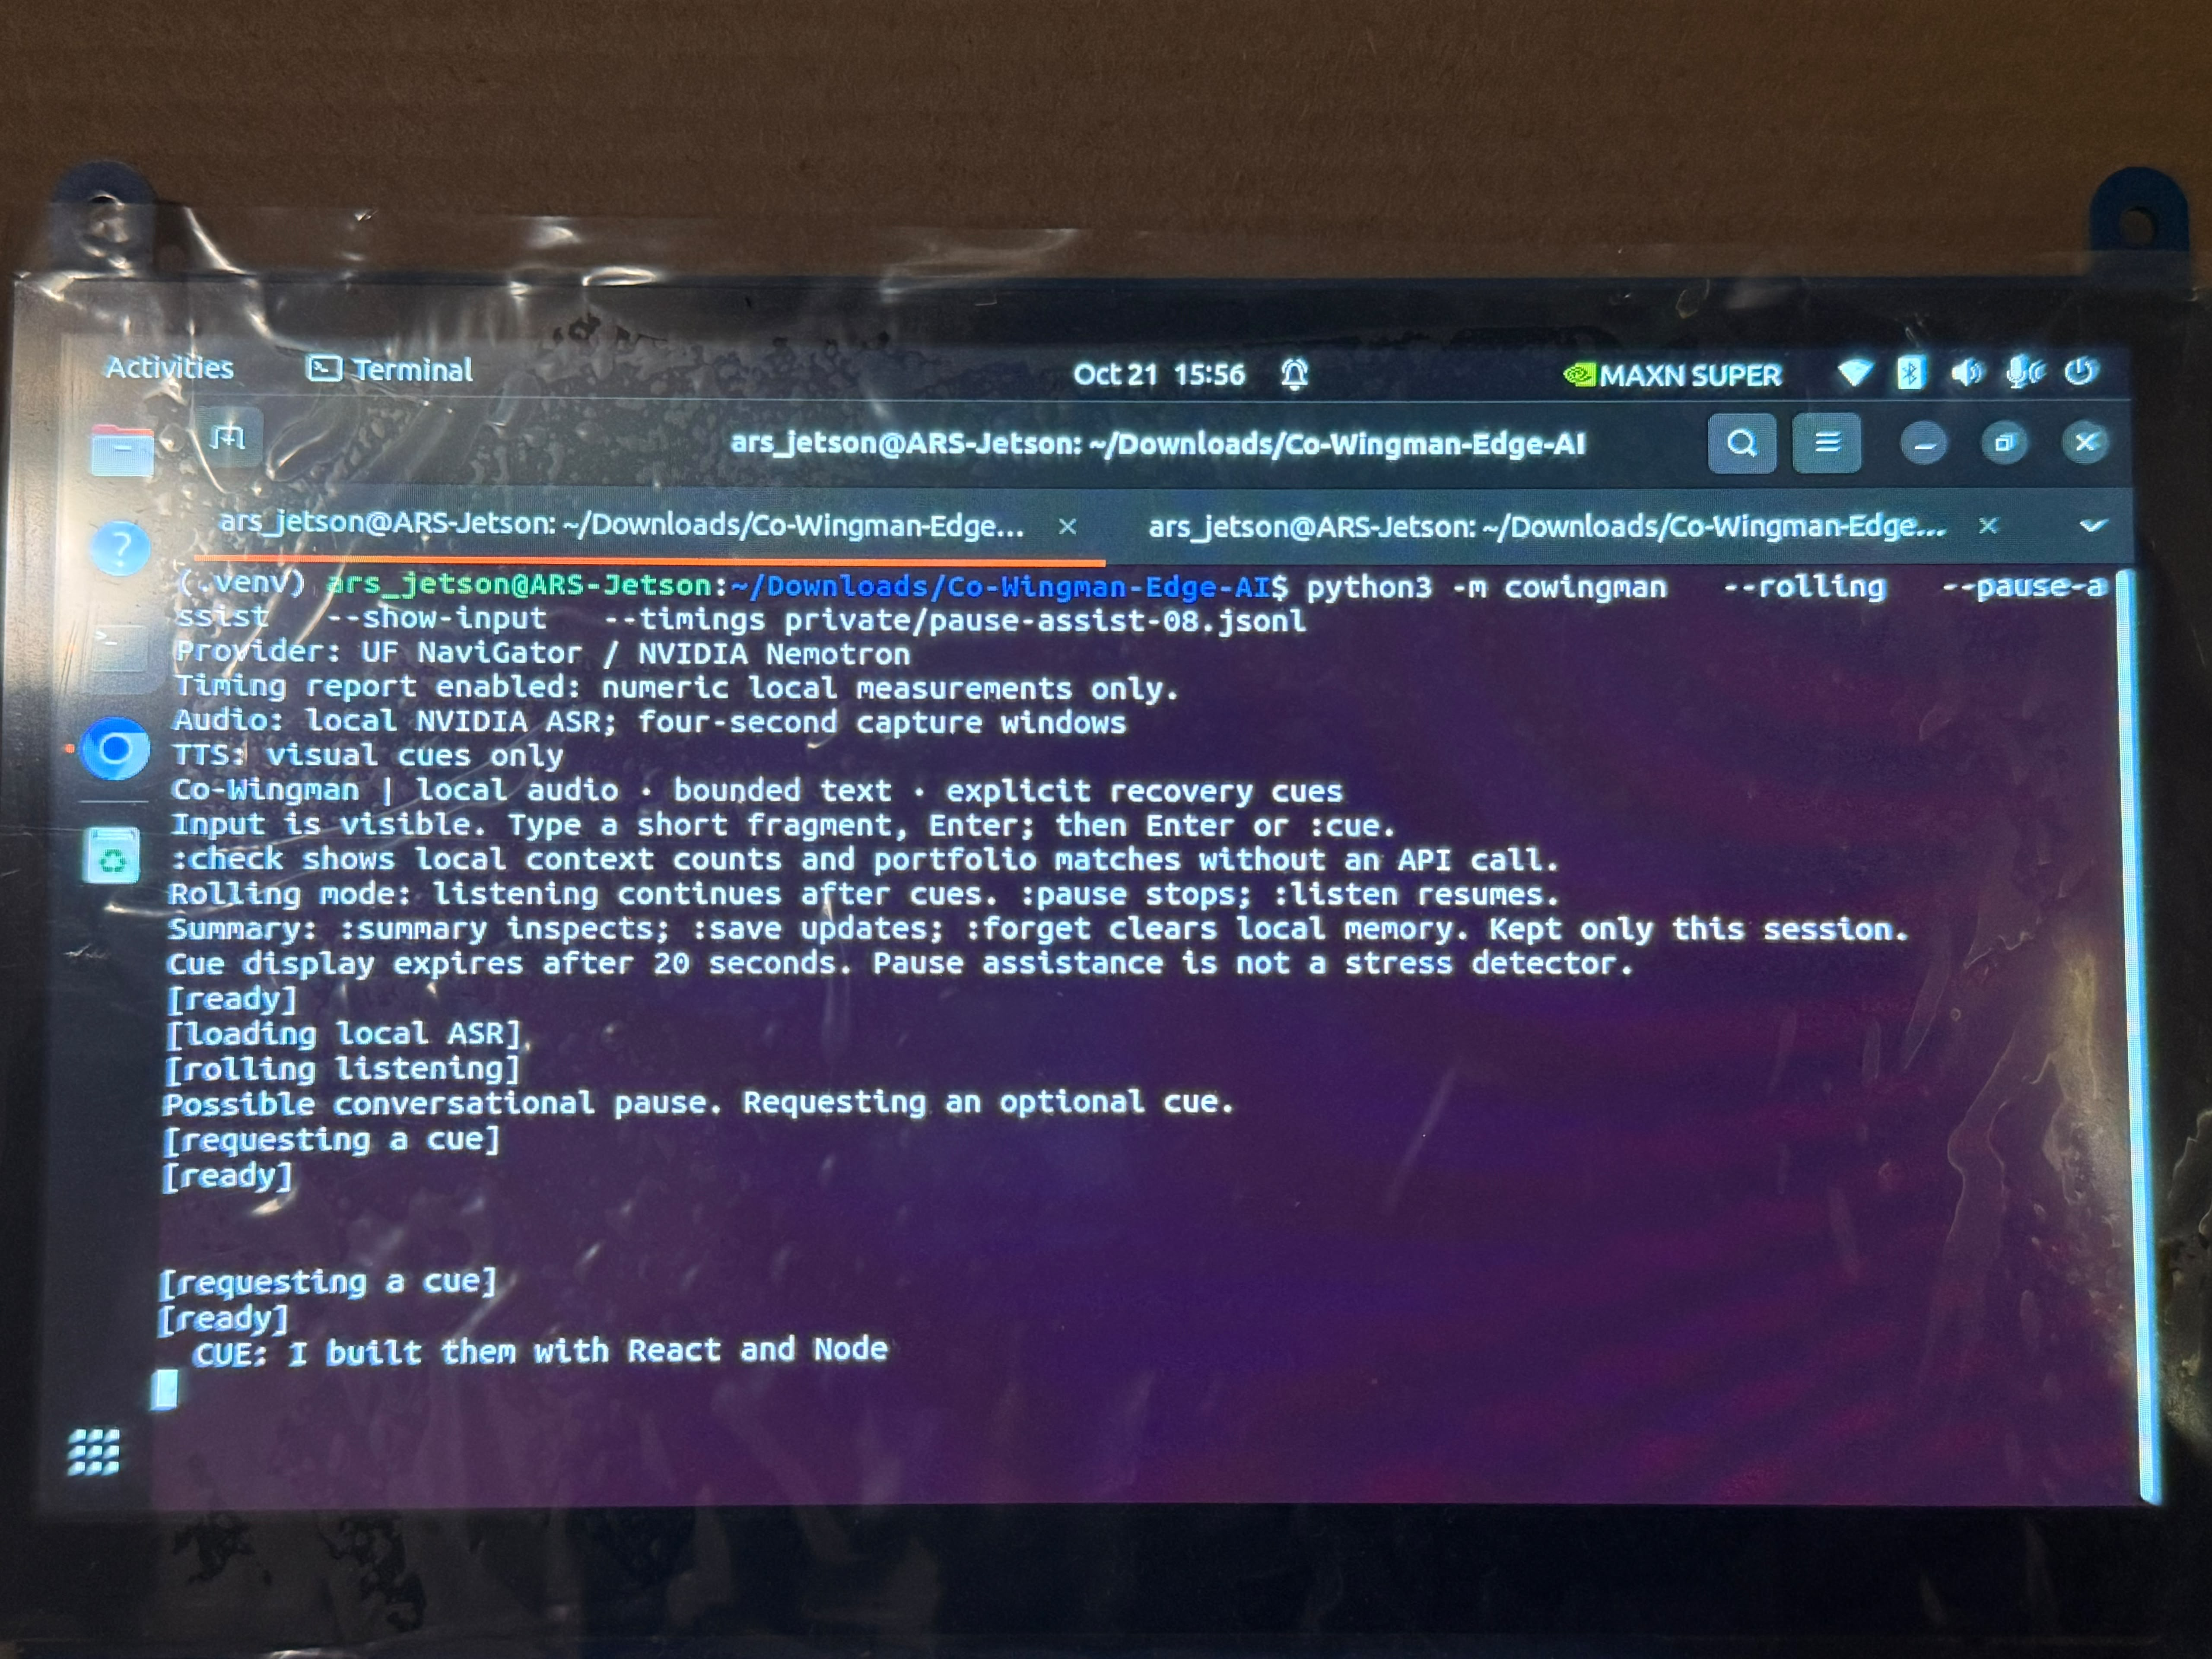
\includegraphics[width=435pt]{images/jetson-output.png}};
\end{scope}
\Text{1032}{489}{390}{17}{ink}{\centering\bfseries Live visual cue demonstrated on Jetson}
\filldraw[rounded corners=5pt,fill=localbg,draw=blue,line width=.6pt]
  (1038,522) rectangle (1418,555);
\Text{1043}{531}{370}{15}{navy}{\centering CUE: I built them with React and Node}

\foreach \x/\value/\label/\col in {
  1028/94/audio windows/navy,
  1164/13/cue requests/orange,
  1300/0/dropped windows/green}{
  \filldraw[rounded corners=6pt,fill=white,draw=lineblue,line width=.8pt]
    (\x,568) rectangle ({\x+128},637);
  \Text{\x+5}{575}{118}{38}{\col}{\centering\bfseries \value}
  \Text{\x+3}{618}{122}{14}{ink}{\centering \label}
}

% The data table is ordinary LaTeX, not an embedded screenshot.
\node[anchor=north west,inner sep=0pt,text=ink] at (1028,648) {%
  \fontsize{14}{17}\selectfont
  \renewcommand{\arraystretch}{1.3}
  \setlength{\tabcolsep}{7pt}
  \begin{tabular}{@{}p{174pt}p{91pt}p{91pt}@{}}
    \hline
    \bfseries Measured stage & \bfseries Median & \bfseries p95\\\hline
    \ResultsRows
    \hline
  \end{tabular}};
\Text{1029}{756}{398}{12}{muted}{\ResultsNote}
\filldraw[rounded corners=6pt,fill=localbg,draw=lineblue]
  (1028,817) rectangle (1428,861);
\Text{1041}{827}{374}{13}{ink}{\AWSStatus}

\Panel{1020}{881}{416}{150}{Next steps}
\Text{1038}{932}{381}{15}{ink}{\NextSteps}

% ---------- FOOTER ----------
\fill[navy] (0,1041) rectangle (1448,1086);
\Text{22}{1054}{1010}{20}{white}{\bfseries Local speech processing\quad
  {\color{orange}\textbullet}\quad Bounded cloud reasoning\quad
  {\color{orange}\textbullet}\quad Optional persistent memory}
\Text{1081}{1058}{345}{12}{white}{\raggedleft
  \href{https://github.com/Co-Wingman-AI/Co-Wingman-Edge-AI}
  {github.com/Co-Wingman-AI/Co-Wingman-Edge-AI}}
\end{tikzpicture}%
}};
\end{tikzpicture}
\end{document}
